\renewcommand*{\arraystretch}{1.5}
\noindent\begin{tabularx}{17cm}{|p{1.95cm}|X|}
	\hline
	number      & 23                                                          \\ \hline
	title       & Holiday destinations                                                           \\ \hline
	\multicolumn{2}{|c|}{ 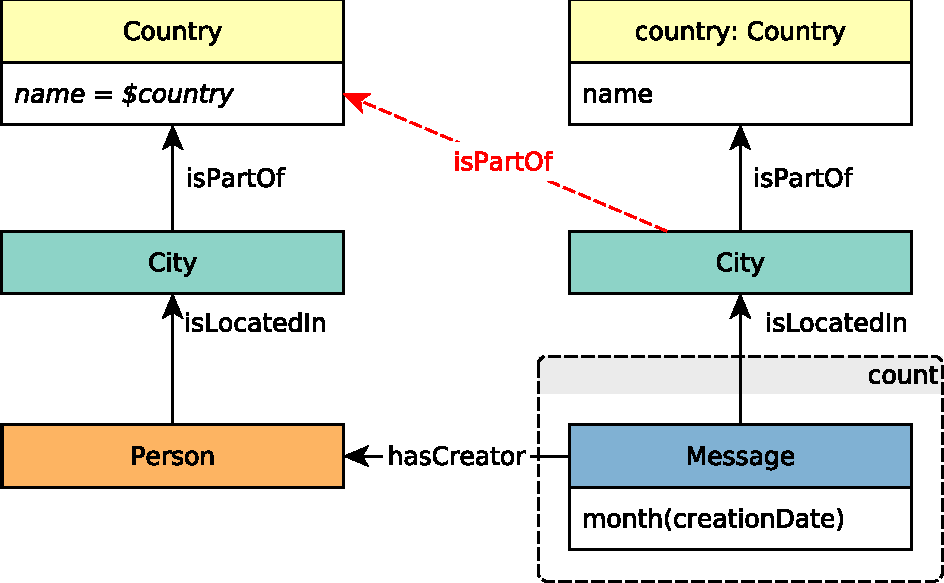
\includegraphics[scale=\patternscale,margin=0cm .2cm]{patterns/q23}} \\ \hline
	description & Count the messages all residents of Country \texttt{country} have
written abroad grouped by month and Country. A Message was written
abroad if the Country the Message was written in is different than the
Country of the Person it was written by.
 \\ \hline
	
	parameters  &
	\renewcommand*{\arraystretch}{1.0}
	\vspace{-1.8ex}{\begin{tabularx}{14.2cm}{|c|l|p{2cm}|Y|} \hline
	\cellcolor{black!70} \color{white} $\mathsf{ 1 }$ & \varname{country} & \cellcolor{gray!20} \vartype{String} & \\ 
	\end{tabularx}} \\ \hline
	result      &
	\renewcommand*{\arraystretch}{1.0}
	\vspace{-1.8ex}{\begin{tabularx}{14.2cm}{|c|l|p{2cm}|Y|} \hline
	\cellcolor{black!70} \color{white} $\mathsf{ 1 }$ & \varname{messageCount} & \cellcolor{gray!20} \vartype{32bitInteger} &The number of messages in each group \\ \hline
	\cellcolor{black!70} \color{white} $\mathsf{ 2 }$ & \varname{country.name} & \cellcolor{gray!20} \vartype{String} &The name of the destination country \\ \hline
	\cellcolor{black!70} \color{white} $\mathsf{ 3 }$ & \varname{month} & \cellcolor{gray!20} \vartype{32bitInteger} & \\ 
	\end{tabularx}} \\ \hline
	sort        &
	\renewcommand*{\arraystretch}{1.0}
	\vspace{-1.8ex}{\begin{tabular}{|c|l|c|} \hline
	\cellcolor{black!70} \color{white} $\mathsf{ 1 }$ & \varname{messageCount} & \cellcolor{gray!20} $\desc$ \\ \hline
	\cellcolor{black!70} \color{white} $\mathsf{ 2 }$ & \varname{country.name} & \cellcolor{gray!20} $\asc$ \\ \hline
	\cellcolor{black!70} \color{white} $\mathsf{ 3 }$ & \varname{month} & \cellcolor{gray!20} $\asc$ \\ 
	\end{tabular}} \\ \hline
	limit       & 100                                                           \\ \hline
	choke points        &
	\multicolumn{1}{>{\raggedright}X|}{
		\chokepoint{1.6}, 
		\chokepoint{2.3}, 
		\chokepoint{2.4}, 
		\chokepoint{3.3}, 
		\chokepoint{4.3}
		}\\ \hline
\end{tabularx}
\clearpage